% !TeX root=main.tex
\pagenumbering{arabic}

\chapter{مقدمه}
\thispagestyle{empty}
\section{مقدمه}
در حال حاضر، یادگیری عمیق
\LTRfootnote{Deep Learning}
به همراه سایر روش‌های یادگیری ماشین 
\LTRfootnote{Machine Learning}
و هوش مصنوعی 
\LTRfootnote{Artificial Intelligence}
پیشرفت‌های چشمگیری در راه‌حل‌های سوال‌ها ارائه داده است به صورتی که برای کدگشایی و حل مسئله‌های سخت علمی با مقیاس بزرگ به طور مثال در بازسازی مدار‌های مغزی
\LTRfootnote{Reconstruction of Brain Circuits}
\cite{Helmstaedter2013ConnectomicRO}
، آنالیز و بررسی جهش‌های DNA 
\LTRfootnote{Analysis of Mutations in DNA}
\cite{Xiong2015TheHS}
از این روش‌ها استفاده می‌شود. علاوه بر این، شبکه‌های عصبی عمیق
\LTRfootnote{\lr{Deep Neural Networks}}
گزینه‌ی مورد علاقه پژوهشگران در هنگام حل بسیاری از مسئله‌های چالش برانگیز در تشخیص صدا و صحبت
\LTRfootnote{Speech Recognition}
\cite{Hinton2012DeepNN}
، متوجه شدن زبان‌ طبیعی
\LTRfootnote{Natural Language Understanding}
\cite{Sutskever2014SequenceTS}
و بینایی ماشین
\LTRfootnote{Computer Vision}
هستند. 
\\
مواردی به مانند پیشرفت مداوم مدل‌های شبکه‌های عصبی عمیق
\cite{Szegedy2016RethinkingTI}, \cite{He2016DeepRL}
، دسترسی باز
\LTRfootnote{Open Access} \cite{Vedaldi2015MatConvNetCN}, \cite{Jia2014CaffeCA}, \cite{Abadi2016TensorFlowLM}
 به کتابخانه‌های نرم‌افزاری یادگیری عمیق و دسترسی آسان به سخت‌افزار‌های مورد نیاز برای آموزش مدل‌های پیچیده کمک کرده‌اند تا یادگیری عمیق به سرعت به حدی از پختگی برای ورود به کاربرد‌های حساس و مهم امنیت  و ایمنی  مانند ماشین‌های خودران
\LTRfootnote{Self Driving Cars}
، سیستم‌های دیدبانی و مراقبت
\LTRfootnote{Surveillance} \cite{Najafabadi2014DeepLA}
، شناسایی بدافزار‌ها
\LTRfootnote{Male-ware Detection} \cite{Papernot2016TowardsTS}, \cite{Grosse2017AdversarialEF}
، ربات‌ها و هواپیماهای بدون سرنشین
\LTRfootnote{Robotics and Drones} \cite{Mnih2015HumanlevelCT}, \cite{Giusti2016AML}
، تشخیص دستور‌های صوتی
\LTRfootnote{Voice Command Recognition} \cite{Hinton2012DeepNN}
 و امنیت شناسایی چهره 
\LTRfootnote{Face ID Security}
 بر روی گوشی همراه برسد. 
\\
این کاربرد‌ها در برخی موارد به حدی اهمیت دارند که جان و مال فرد به آن وابسته می‌شود 
\cite{Madry2018TowardsDL}
و به طور مثال یک حمله‌کننده می‌تواند یک ماشین با راننده اتوماتیک
\LTRfootnote{Autonomous Driving Vehicles}
را گمراه کند یا کنترل عامل‌های هوشمندی که با صدا کنترل ‌می‌شوند
\LTRfootnote{Voice Controlled Intelligent Agents}
را به دست بگیرد. پژوهش‌هایی صورت گرفته که نشان می‌دهد الگوریتم‌های یادگیری ماشین نسبت به نمونه‌های تقابلی
\LTRfootnote{Adversarial Examples}
آسیب‌پذیر هستند. این نمونه‌ها، که با دستکاری‌های
\LTRfootnote{Perturbations}
جزئی و نامحسوس در نمونه‌های مجموعه داده بدست می‌آیند، می‌توانند مدل دسته‌بندی کننده
\LTRfootnote{Classifiers}
را به اشتباه بیندازند. 
\cite{Akhtar2018ThreatOA}
\\
با توجه به اینکه در بیشتر پژوهش‌ها هدف‌ افزایش دقت شبکه بوده و به امنیت و انعطاف‌پذیری  مدل توجهی نشده است یا توجه کمی شده است. بنابراین حتی برای قدرتمند‌ترین شبکه‌های آموزش دیده‌شده که دقت بسیار بالایی در دسته‌بندی تصاویر گزارش می‌دهند، می‌توان به نمونه‌های تقابلی‌ای دست یافت که شبکه را به سمت پیش‌بینی‌ای با اطمینان سوق دهد و گمراه ‌کند.
\section{یک مثال از اهمیت کاربرد نمونه تقابلی}
فرض کنید یک ماشین خودران در حال نزدیک شدن به یک تقاطع است و به یک تابلو ایست نزدیک می‌شود و به جای کاهش سرعت، سرعت خود را افزایش می‌دهد و در نتیجه تصادفی رخ می‌دهد. بعدها یک گزارشگر حادثه افشا می‌کند که به تابلو ایست چهار مستطیل چسبیده بودند و باعث شدند که هوش مصنوعی ماشین آن را به اشتباه محدودیت سرعت ۴۵ تشخیص دهد. این مثال واقعی توسط دانشمندان ارائه شده است و آن‌ها در عمل توانستند با قرار دادن برچسب‌هایی بر روی تابلو ایست، سیستم هوش مصنوعی را به اشتباه و بدخوانی بیندازند
\cite{Evtimov2017RobustPA}.
\\
در ‏شکل
\ref{stop_speed}
تصویر سمت چپ با قرار دادن برچسب‌هایی به تصویر سمت راست تبدیل می‌شود. با وجود اینکه این تصاویر به راحتی توسط انسان قابل شناسایی هستند ولی توسط سیستم‌های هوش مصنوعی به جای تابلو ایست، تابلو محدودیت سرعت ۴۵ تشخیص داده ‌می‌شود که این بسیار خطرناک است. 
\cite{Heaven2019DLFool}
\begin{figure}[H]
	\center{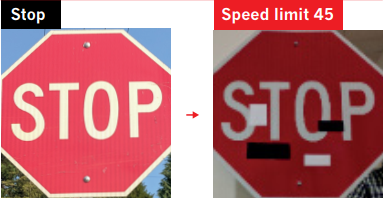
\includegraphics{images/stop_speed.PNG}}
	\caption{نمونه‌ای از خطا شبکه‌های عصبی در تشخیص نشانه‌های راهنمایی و رانندگی
	\cite{Evtimov2017RobustPA}}
	\label{stop_speed}
\end{figure}
